\section{Справочные сведения о походе} 
\subsection{Проводящая организация}
Поход был совершён в рамках школы горного туризма базового уровня, организованной Горной секцией МФТИ.


\subsection{Место проведения}
\textbf{Страна:} Кыргызстан

\textbf{Район:} Центральный Тянь-Шань

\textbf{Подрайон:} Хребет Тескей-Ала-Тоо


\subsection{Общие справочные сведения о маршруте}

\begin{table}[h!]
	\resizebox{\textwidth}{!}{%
		\begin{tabular}{|c|c|c|cc|c|}
			\hline
			\multirow{2}{*}{\begin{tabular}[c]{@{}c@{}}Дисциплина\\ (вид туризма)\end{tabular}} & \multirow{2}{*}{\begin{tabular}[c]{@{}c@{}}Категория сложности\\ маршрута\end{tabular}} & \multirow{2}{*}{\begin{tabular}[c]{@{}c@{}}Протяжённость\\ активной части, км$^1$\end{tabular}} & \multicolumn{2}{c|}{\begin{tabular}[c]{@{}c@{}}Продолжительность активной\\ части\end{tabular}} & \multirow{2}{*}{Срок проведения}                                   \\ \cline{4-5}
			&                                                                                         &                                                                                             & \multicolumn{1}{c|}{Общая}                            & Ходовых дней                            &                                                                     \\ \hline
			Горный                                                                              & Первая                                                                                  & 121.0                                                                                         & \multicolumn{1}{c|}{11}                               & 11                                      & \begin{tabular}[c]{@{}c@{}}03.08.2025~--\\ 13.08.2025 г.\end{tabular} \\ \hline
		\end{tabular}%
	}
\end{table}
\footnotesize{$^1$ С учётом коэффициента $k=1.2$, без учёта повторно пройденного пути}
\normalsize

\subsection{Подробная нитка маршрута}
\textbf{Заявленная:} кур. Джилысу~--- ФГС~--- д.р. Чон-Кызыл-Суу~--- д.р. Саватор~---  \textbf{пер. Саватор~(1А, 4000)}~--- д.р. Киче-Кызыл-Суу~---  \textbf{пер.~Перемётный (1А, 4026)}~--- д.р. Джукучак~--- \textbf{пер.~Ашутор Западный (1А, 3700)}~--- д.р. Ашукашкасуу~---  д.р. Джууку~---  д.р. Иттиши~---  \textbf{пер. Иттиш ~(1А, 3895)}~---  д.р. Ит-Тиши (юж.)~---   д.р. Кашкасу~---   озёра Кашкасу~---  в. Марс (н/к, 4345)~---  \textbf{пер.~Кашкасу  (1А, 3890)}~--- д.р. Ашукашкасуу~--- д.р. Джууку~--- слияние р. Джууку и Джукучак.

\textbf{Пройденная:} Маршрут пройден без изменений.

\textbf{Андрей Баранов, Андрей Козлов, Иван Никитин} сошли с маршрута на слиянии р. Ашукашкасуу и Джууку. Они прошли перевалы Саватор (1А), Перемётный (1А), Ашутор Западный (1А). Пройдено расстояние $L=49.0~\text{км}$ за 6 ходовых дней.

\begin{figure}[h!tbp]
	\centering
	\includegraphics[width=0.99\linewidth]{pics/maps/map.jpg}
	\caption{Обзорная схема маршрута}
\end{figure}

\newpage
\subsection{Высотный профиль маршрута}

\begin{figure}[h!]
	\centering
	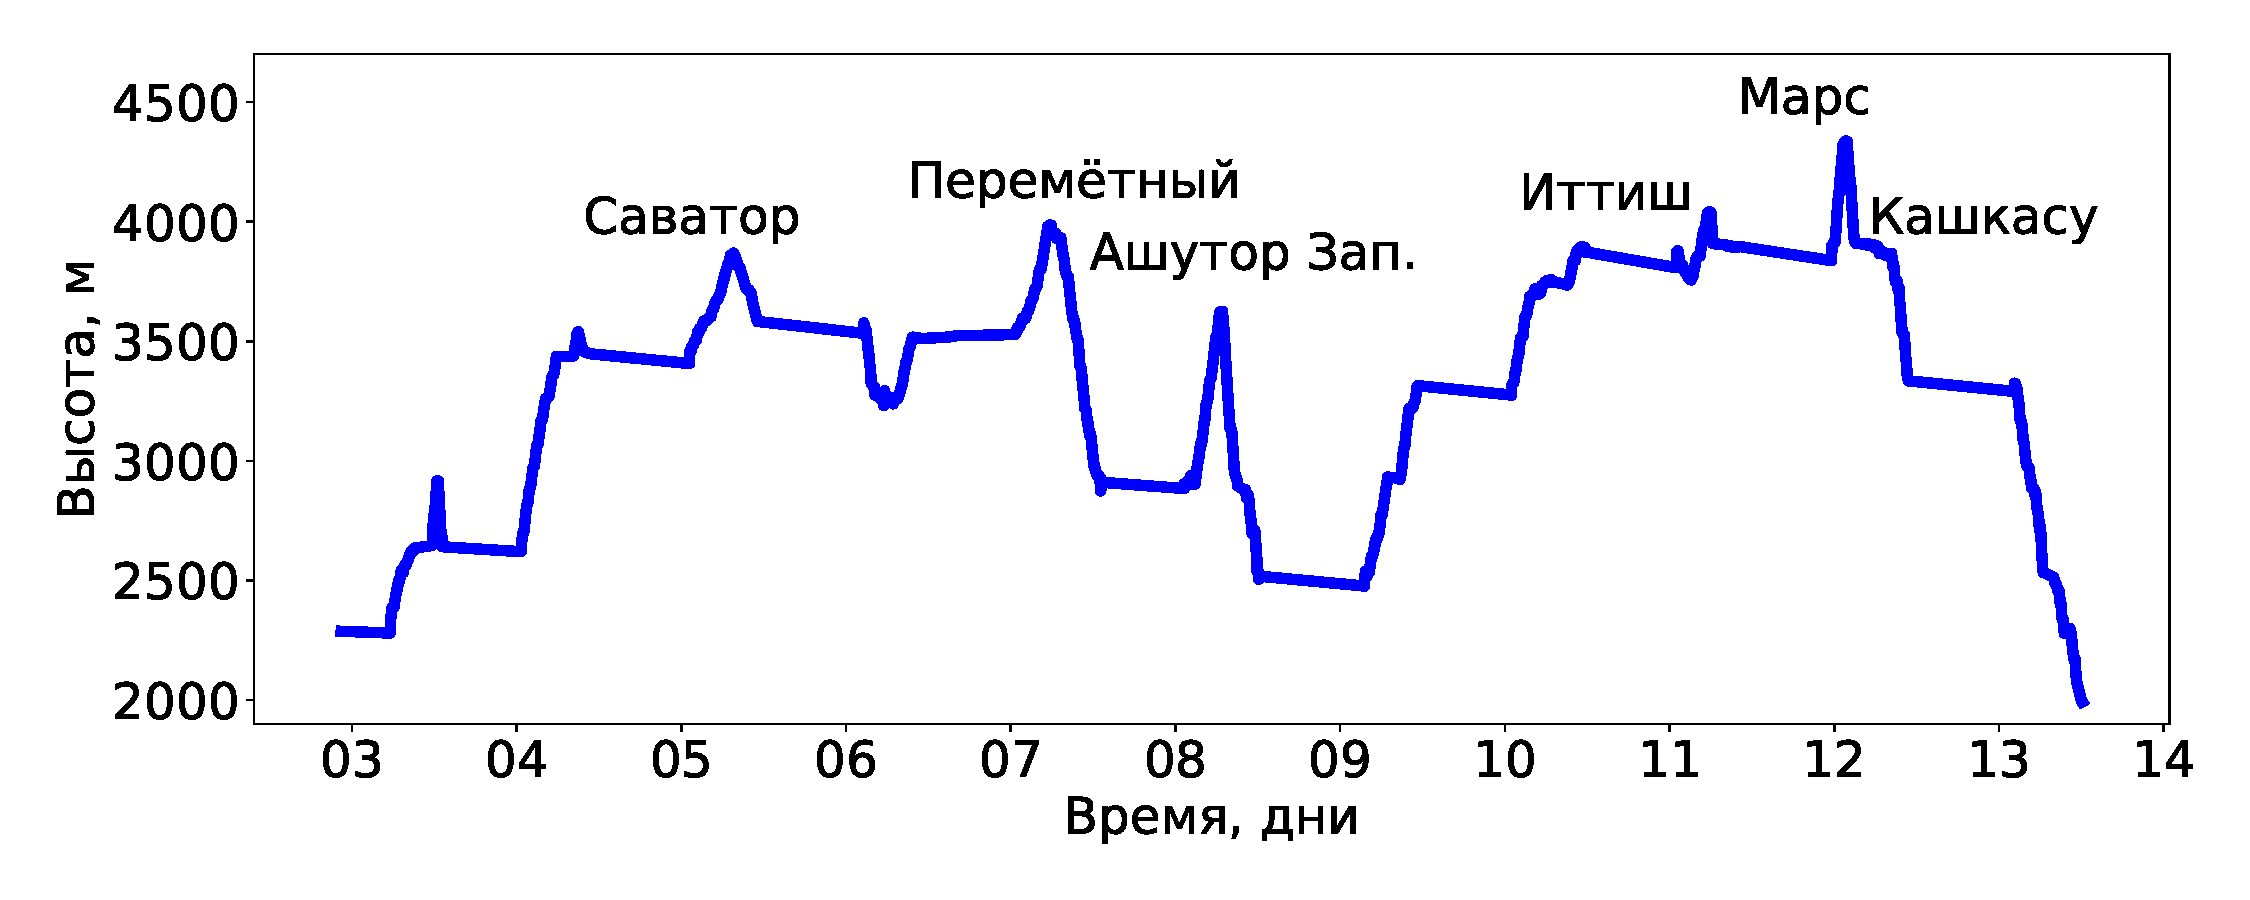
\includegraphics[width=0.92\linewidth]{elevation_vs_time}
	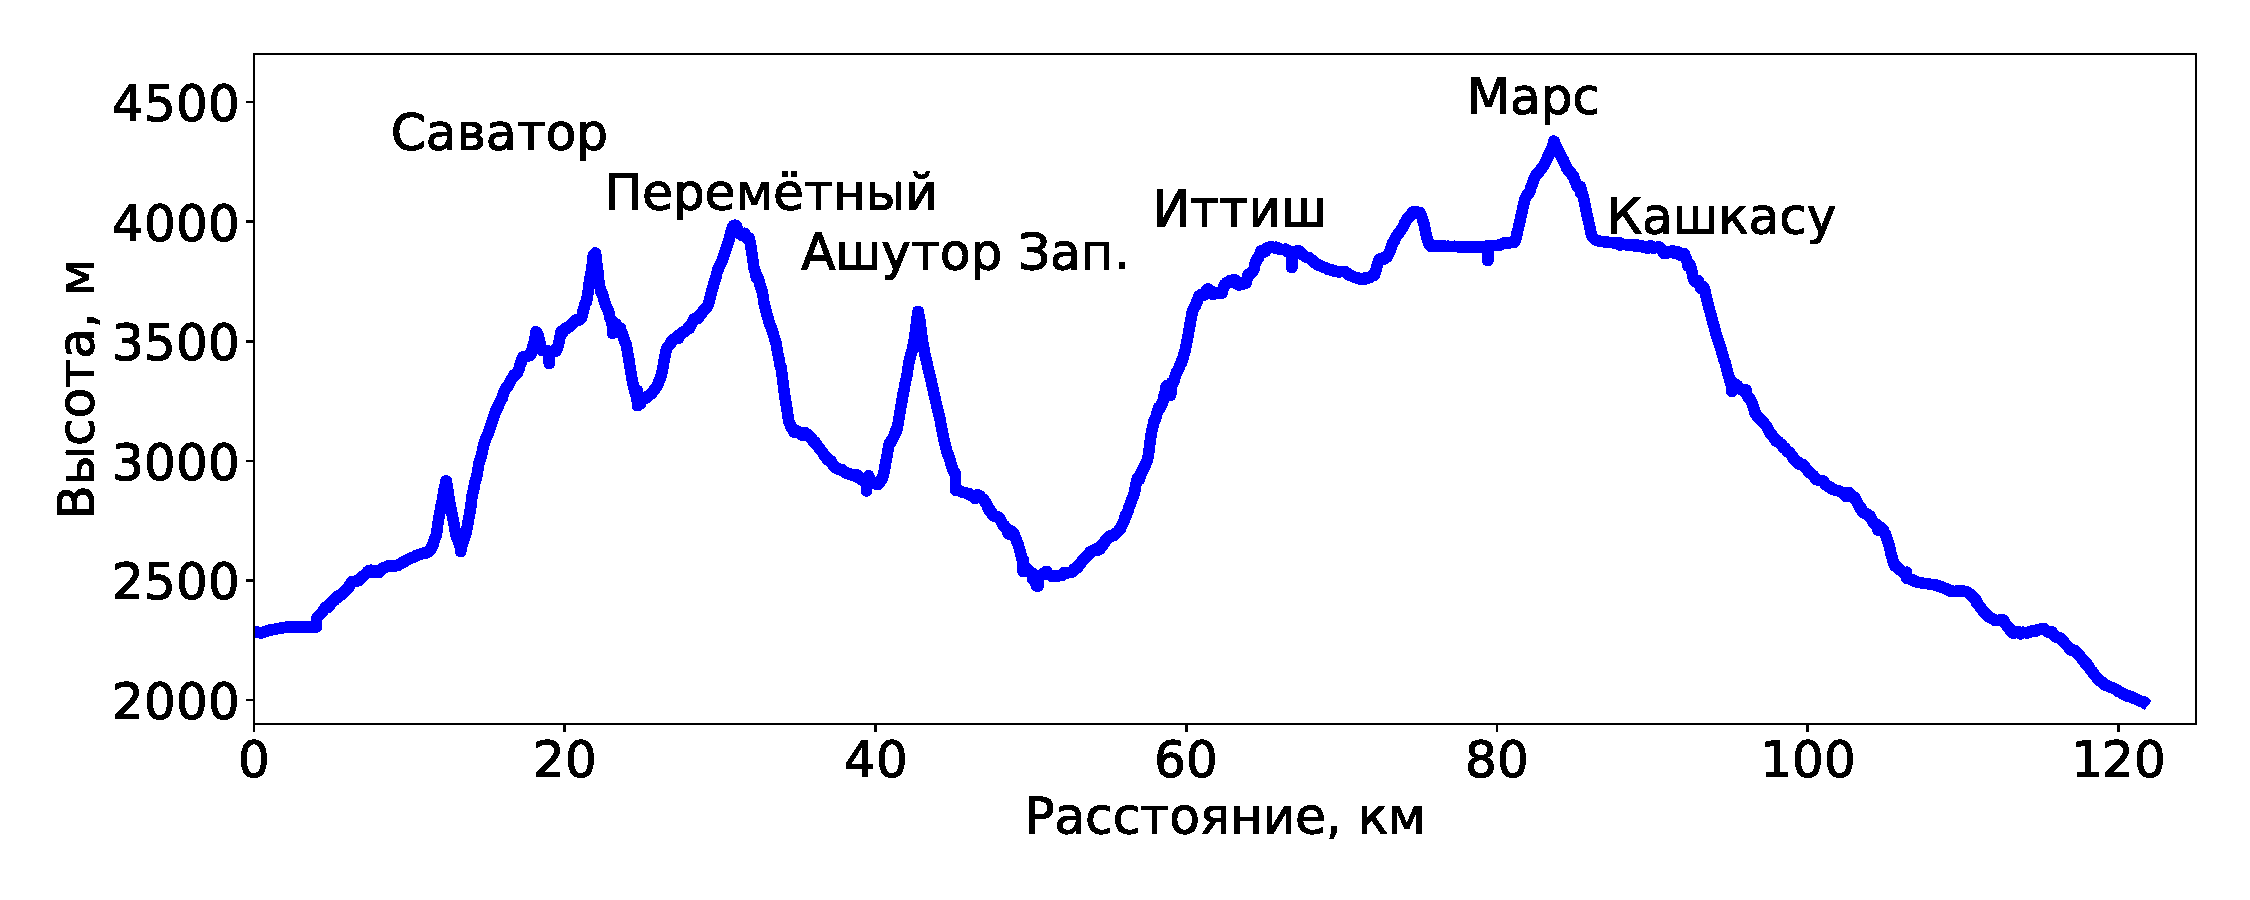
\includegraphics[width=0.92\linewidth]{elevation_vs_distance}
	\caption{Высотный профиль маршрута}
	\label{fig:heights}
\end{figure}

\newpage
\subsection{Определяющие препятствия маршрута}

\begin{table}[h!]
		\begin{tabular}{|>{\centering\arraybackslash}m{0.17\linewidth}|>{\centering\arraybackslash}m{0.03\linewidth}|>{\centering\arraybackslash}m{0.35\linewidth}|>{\centering\arraybackslash}m{0.35\linewidth}|}
			\hline
			\textbf{Вид препятствия, высота} &
			\begin{turn}{90}\textbf{к. тр.}\end{turn} &
			\textbf{Характеристика препятствия на подъём} &
			\textbf{Характеристика препятствия на спуск} \\
			\hline			
			пер. Саватор (4000, по GPS~--- 3860) & 1А &  Со стороны д.р. Саватор тр.-ос. перевальный взлёт протяжённостью до 400 м и крутизной до $30^{\circ}$.  & Со стороны д.р. Киче-Кызыл-Суу ск.-ос., движение до $25^{\circ}$ и протяжённостью до 200 м по крупной и средней осыпи крутизной плотной группой, самостраховка ледорубами, далее~--- по гребню морены и моренному карману.\\
			\hline			
			пер. Перемётный, (4026)  & 1А & Со стороны д.р. Киче-Кызыл-Суу движение по моренному лабиринту, далее по моренным гребням выход на левый пхд борт ледника. Перемётный ледник длиной 1200 м и крутизной  до $15^{\circ}$, движение без кошек. & Движение по перемётному леднику до 300 м  крутизной  до $15^{\circ}$, далее по моренным валам, траверс мелкоосыпного склона протяжённостью до 2 км и крутизной  до $20^{\circ}$ \\
			\hline
			пер. Ашутор Западный (3700)  & 1А & Со стороны д.р. Джукучак по тр.-ос. склону по руслу пересохшего ручья протяжённостью до 300 м, крутизной до $15^{\circ}$, на перевальном взлёте до до $25^{\circ}$. & Движение по границе белой и чёрной мелких осыпей, далее по руслу пересохшего ручья протяжённостью до 150 м., крутизной до $20^{\circ}$\\
			\hline
			пер. Иттиш, (3895)  & 1А & Со стороны д.р. Иттиш движение по ос. гребню протяженностью до 700~м крутизной  до $15^{\circ}$ & Движение по тр. склону протяжённостью до 1000 м и крутизной до $5^{\circ}$\\
			\hline
			пер. Кашкасу, (3890)  & 1А & Со стороны озёр Кашкасу движение по дну ущелья протяжённостью до 2500 м без значительного уклона. &  Движение по гребням морен протяжённостью до 3500 м и уклоном до $15^{\circ}$\\
			\hline
	\end{tabular}%
\end{table}

\clearpage
\subsection{Список участников} 

\begin{table}[h!]
	\centering
	\resizebox{0.82\textwidth}{!}{%
	\begin{tabular}{|>{\centering\arraybackslash}m{0.015\linewidth}|>{\centering\arraybackslash}m{0.14\linewidth}|>{\centering\arraybackslash}m{0.18\linewidth}|>{\centering\arraybackslash}m{0.05\linewidth}|>{\centering\arraybackslash}m{0.15\linewidth}|>{\centering\arraybackslash}m{0.3\linewidth}|}
		\hline
		\textbf{№} &
		\textbf{Фото} &
		\textbf{ФИО} &
		\textbf{г.р.} &
		\textbf{Обязанности в группе} &
		\textbf{Туристский опыт} \\
		\hline			
		
		1	&	\includegraphics[width=0.99\linewidth]{pics/portraits/oa.jpg}	& Остапив Алексей Юрьевич	&	1998	&	Руководитель	& 2ГУ, Киргизский хребет,\newline 3$\times$1ГУ, Кавказ, Алтай \newline 2А тур., 1Б альп.\\
		\hline
		2	& \includegraphics[width=0.99\linewidth]{pics/portraits/dd.jpg}	&Демушкин Дмитрий Юрьевич	&	2001	&	Штурман	& 1ГУ, Кавказ \newline 1А тур.\\
		\hline
		3	&	\includegraphics[width=0.99\linewidth]{pics/portraits/mg.jpg}	&	Герасимова Мария Алексеевна	&	1981	&	Медик	&	\alert{1ГР Кавказ, 2ГУ Кавказ, 1ПУ Крым \newline 1Б тур.} \\
		\hline
		4	&		\includegraphics[width=0.99\linewidth]{pics/portraits/ab.jpg}		&	Баранов Андрей Игоревич	&	1989	&	Финансист	&	1 ст.с., Кавказ \\
		\hline
		5	&	\includegraphics[width=0.99\linewidth]{pics/portraits/ar.jpg}	&	Рогозин Александр Викторович	&	1996	&	Снаряженец	&	1 ст.с. Подмосковье \newline 2Б альп.\\
		\hline
		6	&	\includegraphics[width=0.99\linewidth]{pics/portraits/yuz.jpg}	&	Зернина Юлия Алексеевна	&	2004	&	Завхоз	&	1 ст.с.  Кавказ\\
		\hline
		7	&	\includegraphics[width=0.99\linewidth]{pics/portraits/ak.jpg}	&	Козлов Андрей Викторович	&	2004	&	Реммастер	&	1 ст.с. Подмосковье\\
		\hline
		8	&	\includegraphics[width=0.99\linewidth]{pics/portraits/in.jpg}	&	Никитин Иван Сергеевич	&	2004	&	Фотограф	&	1 ст.с. Подмосковье\\
		\hline
	\end{tabular}%
	}
\end{table}

\clearpage

\subsection{Географическое положение района}

Район Тескей-Ала-Тоо (кырг. <<Пёстрые горы, обращённые от солнца>>)~--- это горный хребет, входящий в горную страну Центрального Тянь-Шаня. Тескей расположен к югу от озера Иссык-Куль, простираясь с запада на восток на 375 км. Средняя высота хребта около 4500 м, высшая точка достирает 5216 м (пик Каракольский).

Крупные узлы оледенения расположены в верховьях рек Чон-Кызылсуу, Джеты-Огуз, Каракол, Арашан, Ак-Суу и Тургень-Ак-Суу. В целом степень оледеления обусловлена высотой и наличием влажного воздуха от Иссык-Куля.

При движении с запада на восток среднегодовое количество осадков увеличивается вдвое, с 1000 мм до 2000 мм (для высокогорья) \cite{rodina2012}. Температура воздуха колеблется летом от -5\degree (сырты, высота 4000 м, август) до 15\degree~(д.р. Джукучак, высота 2500 м, август)

В районе ярко выражена высотная поясность. Зона леса, представленная преимущественно высокими тянь-шаньскими елями, располагается на высотах 2100--3100 м. До высоты 3800 м следует зона альпийских лугов, а снеговая линия в августе находится на высотах от 4000 м (для северных склонов хребта). Южная же сторона хребта представлена заболоченным плоскогорьем~--- сыртами, и как по климату, так и по растительности и рельефу резко контрастирует с северной стороной.

Долины рек, текущих вдоль отрогов главного хребта, широкие, долины их боковых притоков узкие с высокой и крутой устьевой ступенью.

\subsection{Туристские особенности района}
Район очень привлекателен для горных туристов, поскольку в нём представляется возможным проведение горных походов любой к.с.~--- от <<единичек>> до <<шестёрок>>. Этому способствуют несколько факторов: достаточно простая логистика, наличие локальных препятсивий любого уровня сложности в достаточном количества, разнообразие природного рельефа. Уникальной особенностью западной оконечности центрального Тескея (долины рек Джууку, Иттиш, Ашукашкасу, Джукучак) является возможность перехода с северной стороны хребта на южную по перевалам с категорией сложности не выше 1А, чем строго рекомендуется пользоваться при планировании простых горных походов по району.

Самыми посещаемыми долинами являются д.р. Чон-Кызыл-Суу, Джеты-Огуз, Телеты, Каракол. Здесь, помимо спортивных, проходит множество коммерческих маршрутов, можно встретить туристов из Европы и США. Прочие долины, несмотря на хорошую изученность, посещаются значительно реже. Впрочем, стоит отметить сильно возросший интерес к д.р. Джууку, Иттиш, Ашукашкасу, Джукучак после публикации отчёта Д. Ковинова в 2021 году \cite{kovinov2021}.

К дополнительным особенностям района стоит отнести наличие горячих радоновых источников в д.р. Джеты-Огуз, Джукучак.

Типичной погодой для района следует считать ясную теплую первую половину дня и дождливый вечер (как правило, после 15:00) \cite{rodina2012, tipsina2024, sergeev2024, smurov2024}. Это следует обязательно учитывать при планировании ходового дня.

Все долины крупных рек, а также значительная часть их больших боковых притоков используются под высокогорных пастбища со всеми вытекающими последствиями для качества сырой воды.

\clearpage